\subsection{Perch Detection Success Rate}

The results show that the proposed image processing method has potential, though performance is dependent on the background.
Both patterned backgrounds performed worse than the plain white wall, with the checkered pattern performing extremely poorly (not
even a 50\% success rate), and the zigzag background showing a much smaller performance reduction compared to the white wall than 
for the checkered background.

The reason for the difference between the success rate for checkered and zigzag background patterns is not immediately obvious. 
Inspecting the point cloud data for each reveals that the problem most likely lies in how the background pattern is interacting 
with the \texttt{StereoSGBM} block matcher. Fig. \ref{fig:pattern-compare} shows the differences in stereo camera data for two samples
from each background pattern. It shows that the checkered pattern produces a region of erroneous high disparity, which prevents the 
line detection algorithms from correctly selecting the test object. Further experimentation would be needed to determine exactly 
why that is happening, one possibility is that the checker pattern is too small compared to the block size or disparity range
that \texttt{StereoSGBM} was configured to use, leading to incorrect block matches.

\begin{figure}[H]
    \centering
    % Generated from "C:\\Users\\wyatt\\Documents\\GVSU\\Thesis\\august_test_data\\idc_sept_5\\blanket\\pvc_2000_0_0_0_bin_5"
    \begin{subfigure}[b]{\textwidth}        
        \begin{subfigure}[b]{0.32\textwidth}
            \centering
            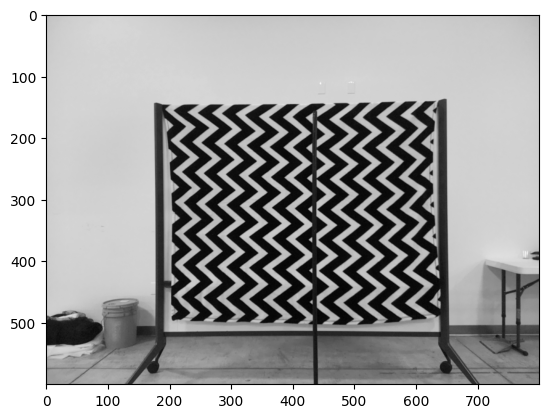
\includegraphics[width=\textwidth]{sections/discussion/zigzag-left-failure.png}
            \caption{Left camera image with zigzag background.}
            \label{fig:pattern-compare:zigzag:img}
        \end{subfigure}
        \hfill
        \begin{subfigure}[b]{0.32\textwidth}
            \centering
            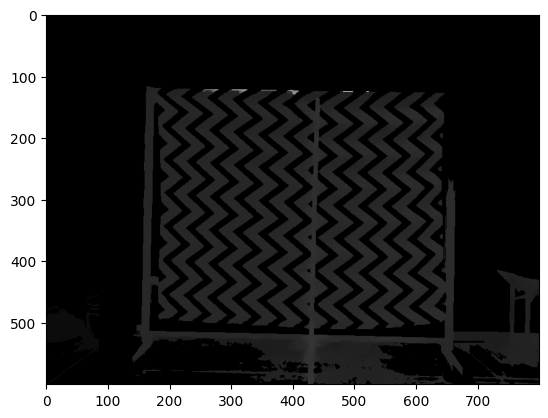
\includegraphics[width=\textwidth]{sections/discussion/zigzag-disp-failure.png}
            \caption{Disparity map calculated from \ref{fig:pattern-compare:zigzag:img} and the corresponding right image.}
            \label{fig:pattern-compare:zigzag:disp}
        \end{subfigure}
        \hfill
        \begin{subfigure}[b]{0.32\textwidth}
            \centering
            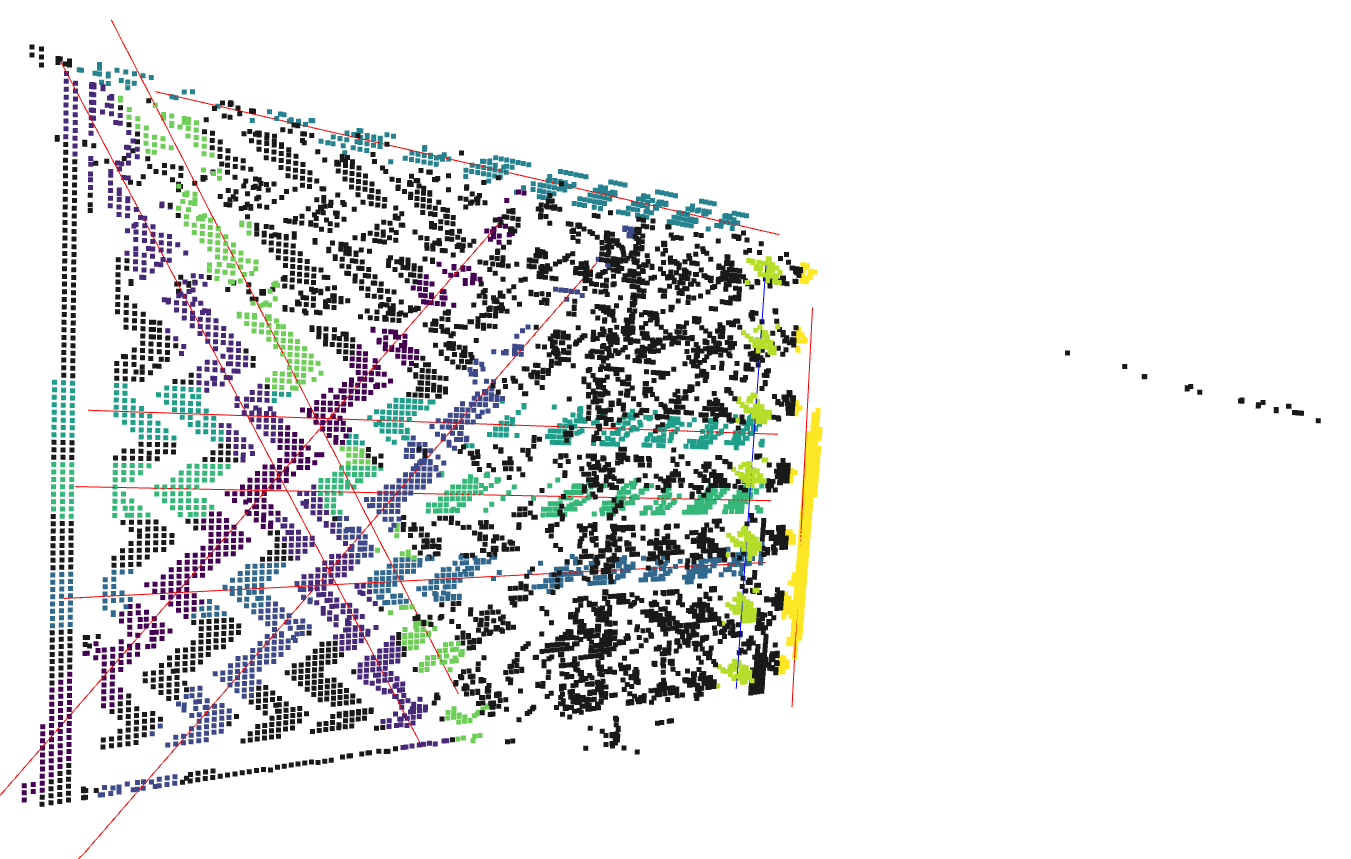
\includegraphics[width=\textwidth]{sections/discussion/zigzag-ptcld-failure.png}
            \caption{Point cloud produced from the disparity data in \ref{fig:pattern-compare:zigzag:disp}.}
            \label{fig:pattern-compare:zigzag:ptcld}
        \end{subfigure}
    \end{subfigure}
    \vfill
    \begin{subfigure}[b]{\textwidth}
        % Generated from "C:\\Users\\wyatt\\Documents\\GVSU\\Thesis\\august_test_data\\idc_sept_5\\cloth\\pvc_2000_0_0_0_bin_18"
        \begin{subfigure}[b]{0.32\textwidth}
            \centering
            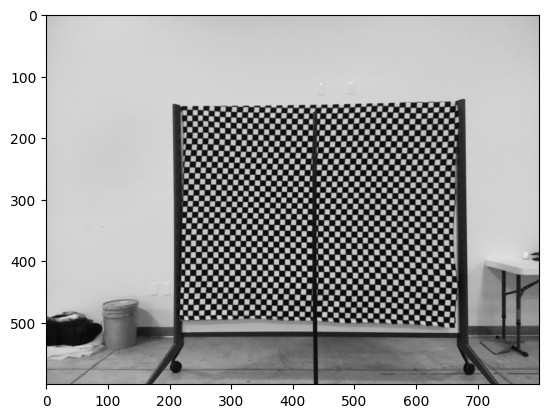
\includegraphics[width=\textwidth]{sections/discussion/check-left-failure.png}
            \caption{Left camera image with checkered background.}
            \label{fig:pattern-compare:check:img}
        \end{subfigure}
        \hfill
        \begin{subfigure}[b]{0.32\textwidth}
            \centering
            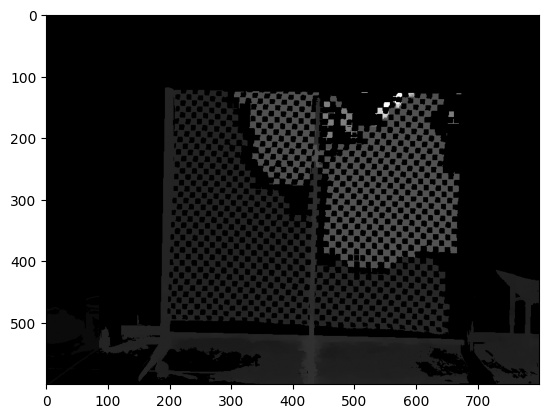
\includegraphics[width=\textwidth]{sections/discussion/check-disp-failure.png}
            \caption{Disparity map calculated from \ref{fig:pattern-compare:check:img} and the corresponding right image.}
            \label{fig:pattern-compare:check:disp}
        \end{subfigure}
        \hfill
        \begin{subfigure}[b]{0.32\textwidth}
            \centering
            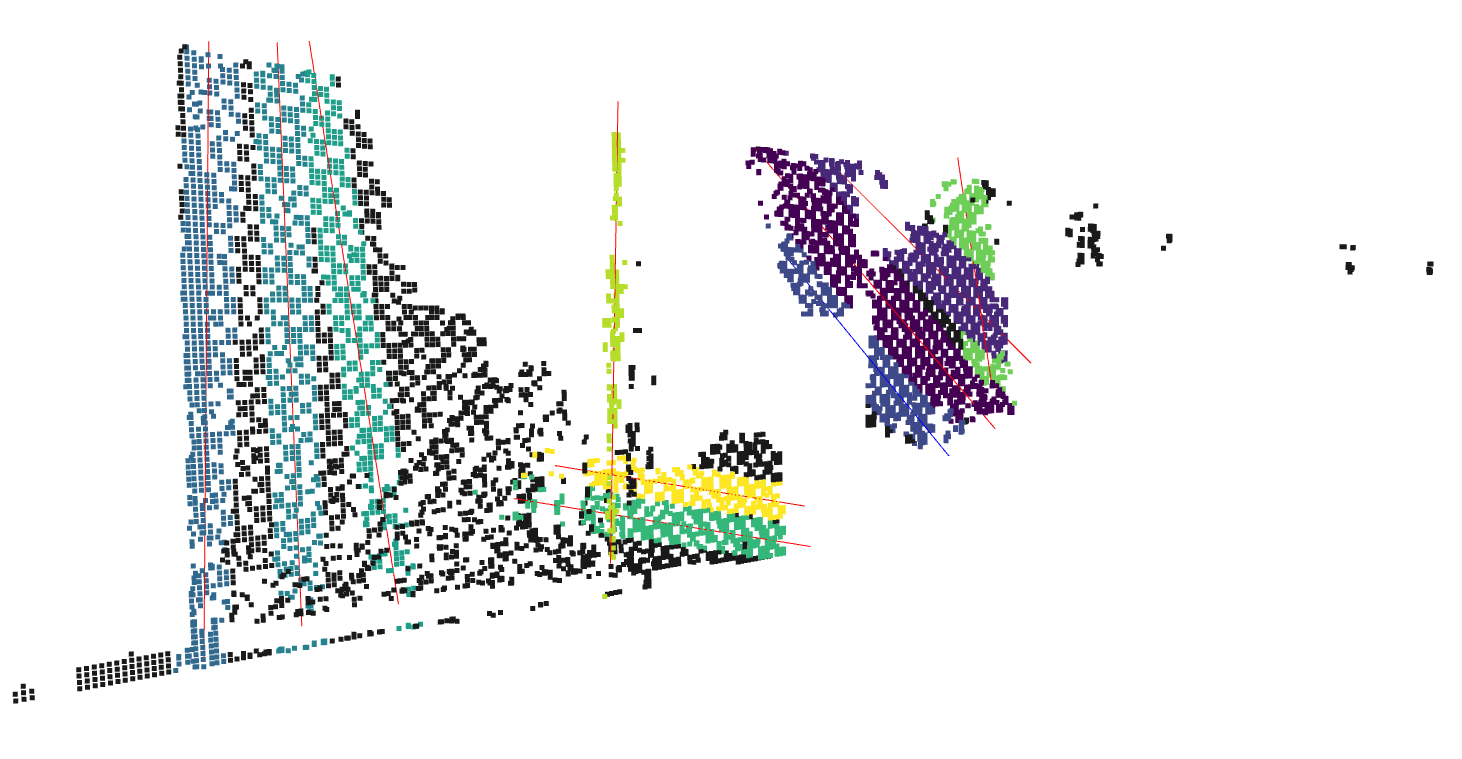
\includegraphics[width=\textwidth]{sections/discussion/check-ptcld-failure.png}
            \caption{Point cloud produced from the disparity data in \ref{fig:pattern-compare:check:disp}.}
            \label{fig:pattern-compare:check:ptcld}
        \end{subfigure}
    \end{subfigure}
    \caption{Comparison of sample data with the zigzag background and the checkered background. In both of the cases shown the object
        was not successfully detected. Note the region of high disparity in the upper right corner of the backdrop shown in \ref{fig:pattern-compare:check:disp},
        which is not seen in \ref{fig:pattern-compare:zigzag:disp}.}
    \label{fig:pattern-compare}
\end{figure}

The failures with the zigzag background do not appear to be a result of incorrect disparity data like the checkered background failures. 
Fig. \ref{fig:zigzag-fail-2} and \ref{fig:zigzag-fail-3} show sample data from two more failure cases with the zigzag background. Neither
Fig. \ref{fig:zigzag-fail-2:disp} nor \ref{fig:zigzag-fail-3:disp} show erroneous disparity artifacts such as seen in Fig. \ref{fig:pattern-compare:check:disp}.
Instead, the failures seem to be related to the Hough line detection. Fig. \ref{fig:zigzag-fail-2:ptcld-front} and \ref{fig:zigzag-fail-3:ptcld-front} 
show that the test object was not even identified as a target line (as it is shown in black and has no line drawn through it). This suggests that
the line did not meet the minimum vote threshold, or it had few enough votes that there were 10 higher voted incorrect lines.
Fig. \ref{fig:zigzag-fail-2:ptcld-side} and \ref{fig:zigzag-fail-3:ptcld-side} show that the test object was split up somewhat in 
the z axis, which may explain why its vote count was low. Lowering the minimum Hough vote threshold or raising the maximum number
of lines could help with this, though could also increase false detections due to poor quality background depth data.


\begin{figure}[H]
    \centering
    % Generated from "C:\\Users\\wyatt\\Documents\\GVSU\\Thesis\\august_test_data\\idc_sept_5\\blanket\\pvc_2000_0_0_0_bin_18"
    \begin{subfigure}[b]{\textwidth}
        \begin{subfigure}[b]{0.45\textwidth}
            \centering
            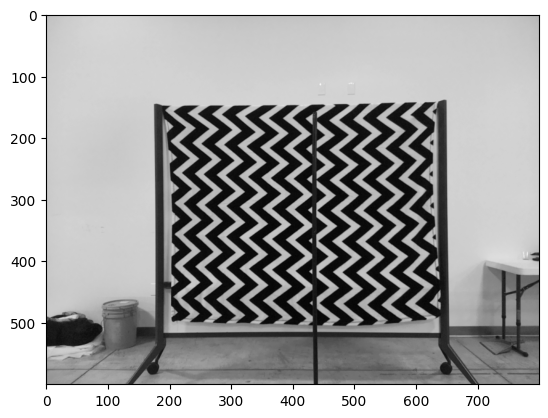
\includegraphics[width=\textwidth]{sections/discussion/zigzag-left-failure-2.png}
            \caption{Left camera image with the zigzag background pattern.}
            \label{fig:zigzag-fail-2:img}
        \end{subfigure}
        \hfill
        \begin{subfigure}[b]{0.45\textwidth}
            \centering
            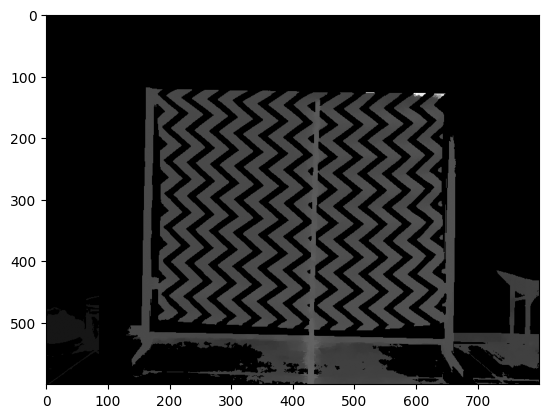
\includegraphics[width=\textwidth]{sections/discussion/zigzag-disp-failure-2.png}
            \caption{Disparity map produced from \ref{fig:zigzag-fail-2:img} and the corresponding right image.}
            \label{fig:zigzag-fail-2:disp}
        \end{subfigure}
    \end{subfigure}
    \vfill
    \begin{subfigure}[b]{\textwidth}
        \begin{subfigure}[b]{0.45\textwidth}
            \centering
            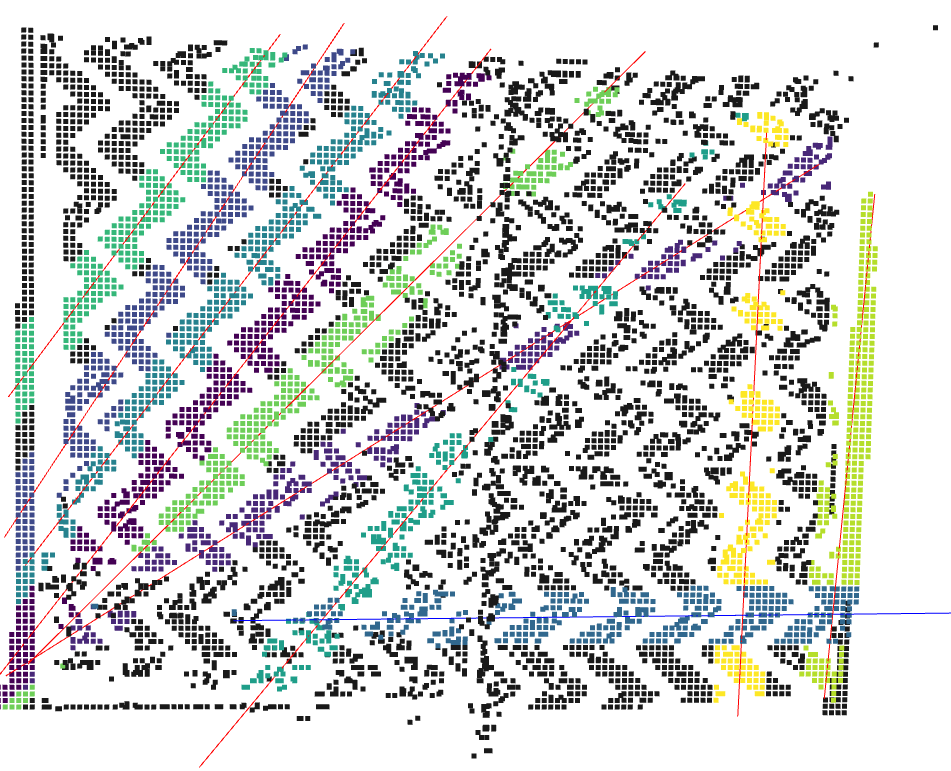
\includegraphics[width=\textwidth]{sections/discussion/zigzag-ptcld-failure-2-front.png}
            \caption{Front view of the point cloud produced from the disparity data in \ref{fig:zigzag-fail-2:disp}.}
            \label{fig:zigzag-fail-2:ptcld-front}
        \end{subfigure}
        \hfill
        \begin{subfigure}[b]{0.45\textwidth}
            \centering
            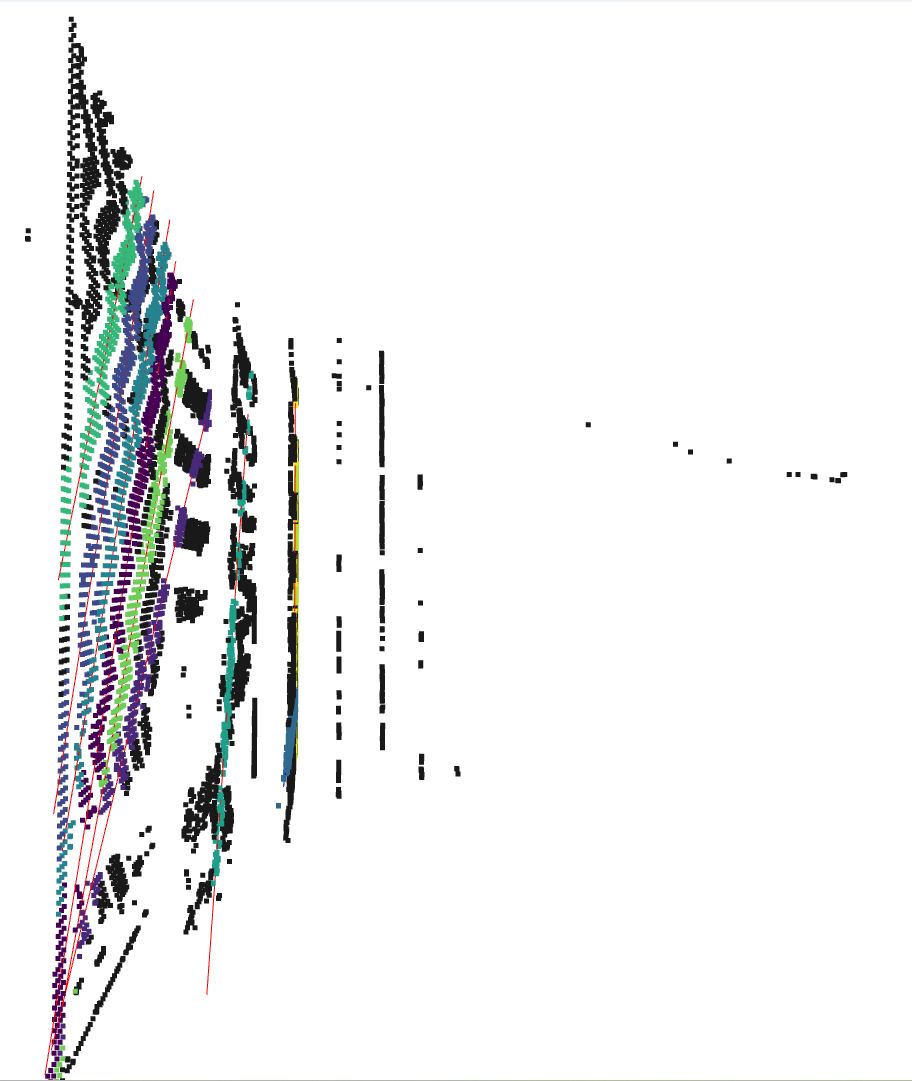
\includegraphics[width=\textwidth]{sections/discussion/zigzag-ptcld-failure-2-side.png}
            \caption{Side view of the same point cloud shown in \ref{fig:zigzag-fail-2:ptcld-front}.}
            \label{fig:zigzag-fail-2:ptcld-side}
        \end{subfigure}
    \end{subfigure}
    \caption{Sample failure case with the zigzag background. Note that the point cloud in \ref{fig:zigzag-fail-2:ptcld-front} and
    \ref{fig:zigzag-fail-2:ptcld-side} shows the test object was not identified as a candidate line.}
    \label{fig:zigzag-fail-2}
\end{figure}


\begin{figure}[H]
    \centering
    % Generated from "C:\\Users\\wyatt\\Documents\\GVSU\\Thesis\\august_test_data\\idc_sept_5\\blanket\\pvc_2000_0_0_0_bin_7"
    \begin{subfigure}[b]{\textwidth}
        \begin{subfigure}[b]{0.45\textwidth}
            \centering
            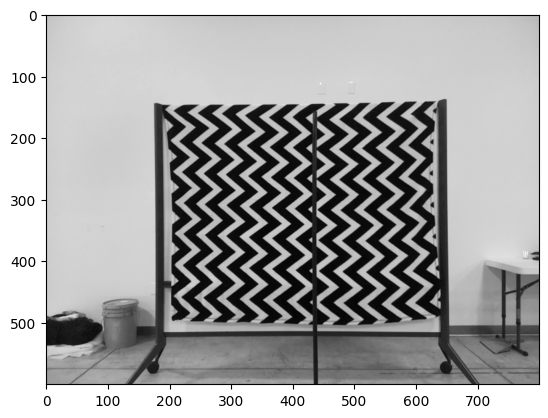
\includegraphics[width=\textwidth]{sections/discussion/zigzag-left-failure-3.png}
            \caption{Left camera image with the zigzag background pattern.}
            \label{fig:zigzag-fail-3:img}
        \end{subfigure}
        \hfill
        \begin{subfigure}[b]{0.45\textwidth}
            \centering
            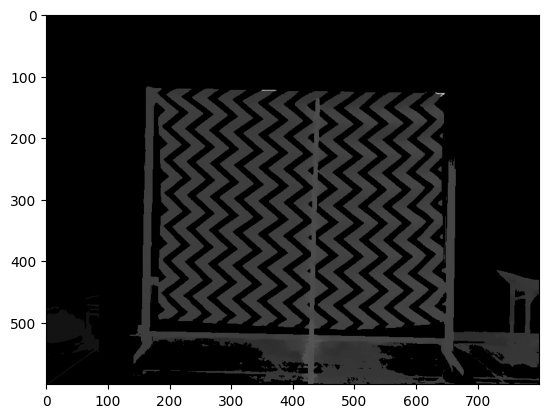
\includegraphics[width=\textwidth]{sections/discussion/zigzag-disp-failure-3.png}
            \caption{Disparity map produced from \ref{fig:zigzag-fail-3:img} and the corresponding right image.}
            \label{fig:zigzag-fail-3:disp}
        \end{subfigure}
    \end{subfigure}
    \vfill
    \begin{subfigure}[b]{\textwidth}
        \begin{subfigure}[b]{0.45\textwidth}
            \centering
            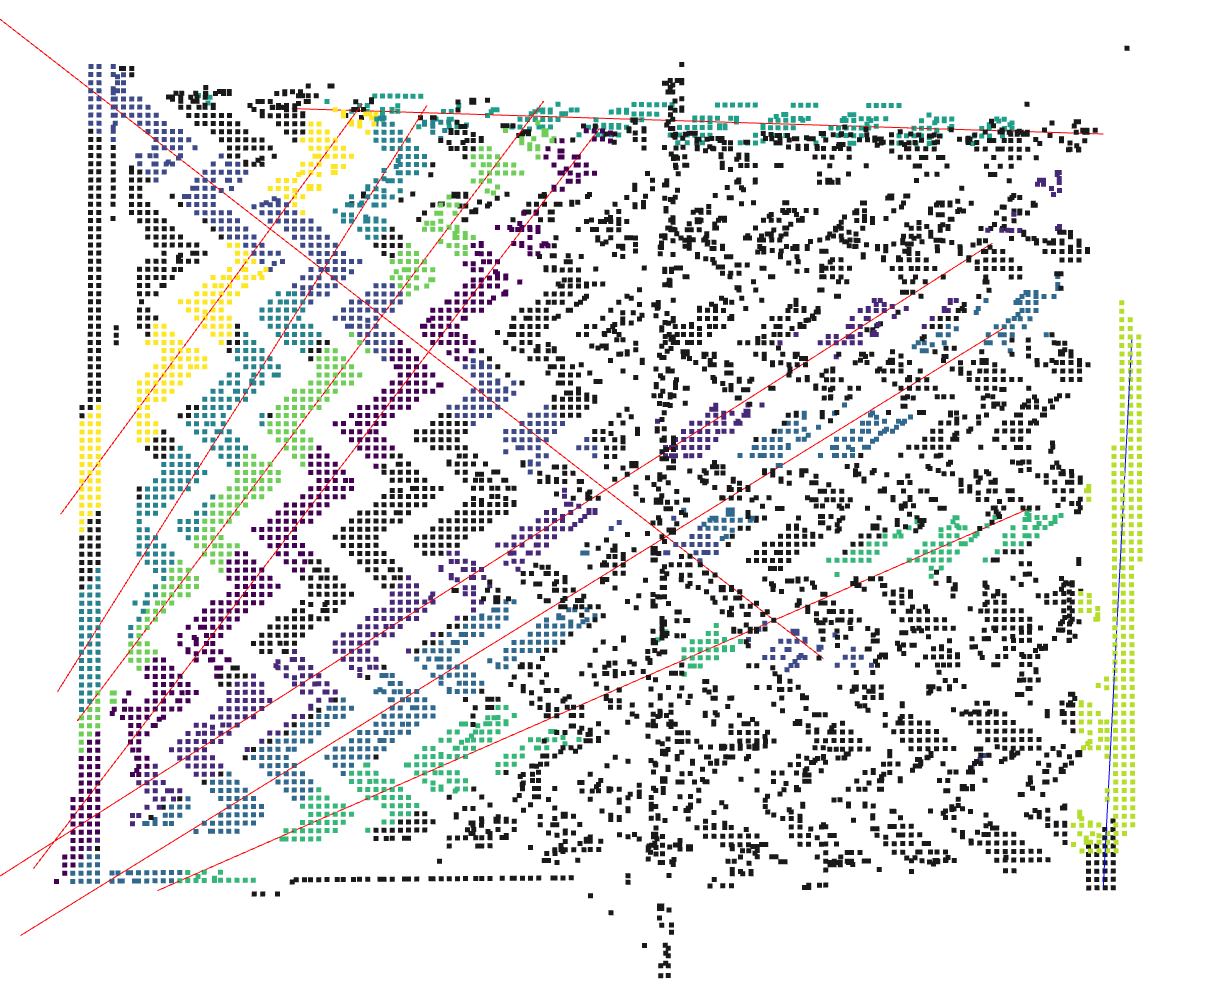
\includegraphics[width=\textwidth]{sections/discussion/zigzag-ptcld-failure-3-front.png}
            \caption{Front view of the point cloud produced from the disparity data in \ref{fig:zigzag-fail-3:disp}.}
            \label{fig:zigzag-fail-3:ptcld-front}
        \end{subfigure}
        \hfill
        \begin{subfigure}[b]{0.45\textwidth}
            \centering
            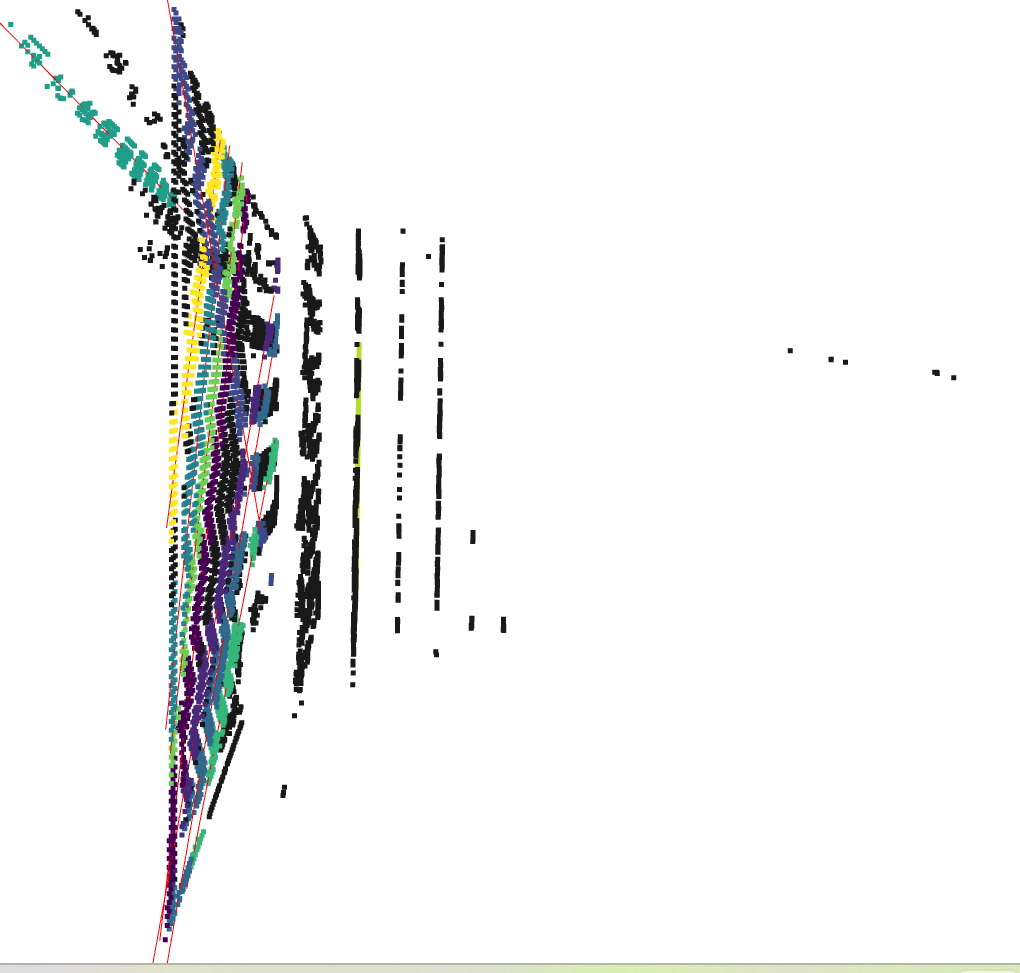
\includegraphics[width=\textwidth]{sections/discussion/zigzag-ptcld-failure-3-side.png}
            \caption{Side view of the same point cloud shown in \ref{fig:zigzag-fail-3:ptcld-front}.}
            \label{fig:zigzag-fail-3:ptcld-side}
        \end{subfigure}
    \end{subfigure}
    \caption{Sample failure case with the zigzag background. Note that the point cloud in \ref{fig:zigzag-fail-3:ptcld-front} and
    \ref{fig:zigzag-fail-3:ptcld-side} shows the test object was not identified as a candidate line.}
    \label{fig:zigzag-fail-3}
\end{figure}


\subsection{Multiple Object Success Rate}

Table \ref{tab:success-rates-dist-multi} shows that, against the flat white background, adding a second object behind the first did not
impact the success rate. The checkered background does not show a significant difference (p > 0.05 via Chi-Squared test with 1 degree of freedom)
between the results with one or two objects. 

The results for the zigzag backdrop do display a significant change in success rate, interestingly an increase. 
Inspecting the results showed that issues such as illustrated in Fig. \ref{fig:zigzag-fail-2} and \ref{fig:zigzag-fail-3},
where the test object is not recognized as a line in the point cloud, did not happen as often when the second object was added.
Fig. \ref{fig:zigzag-2obj-compare} illustrates the difference between sample point clouds with one and two objects. 

How the addition of the second object could have improved the overall point cloud quality and increased the successful 
detection rate is not clear; it may be that this change was instead caused by slight variation in the backdrop placement
between these two tests or other uncontrolled variables.


\begin{figure}[H]
    \centering
    % Generated from "C:\\Users\\wyatt\\Documents\\GVSU\\Thesis\\august_test_data\\idc_sept_5\\blanket\\pvc_2000_0_0_0_bin_18"
    \begin{subfigure}[b]{\textwidth}
        \begin{subfigure}[b]{0.45\textwidth}
            \centering
            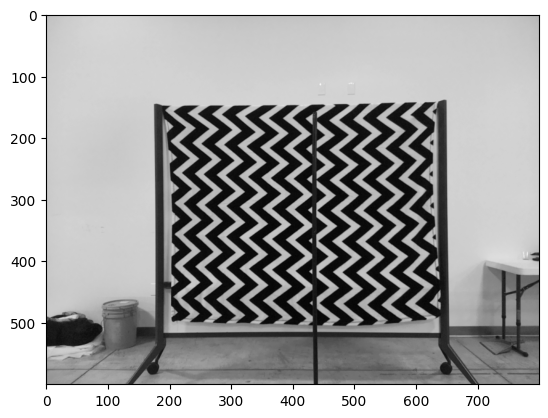
\includegraphics[width=\textwidth]{sections/discussion/zigzag-left-failure-4.png}
            \caption{Left camera image with a single test object.}
            \label{fig:zigzag-2obj-compare:left-single}
        \end{subfigure}
        \hfill
        \begin{subfigure}[b]{0.45\textwidth}
            \centering
            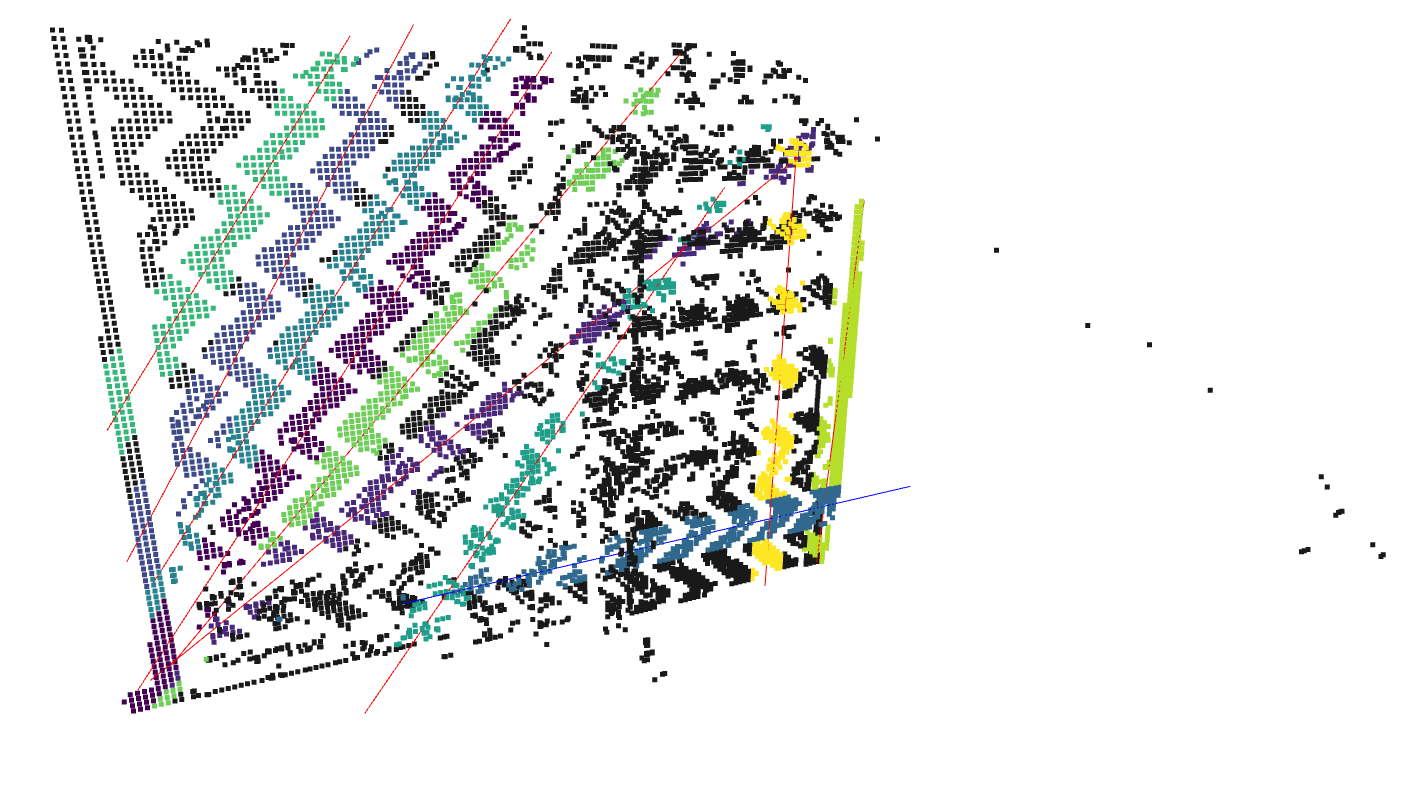
\includegraphics[width=\textwidth]{sections/discussion/zigzag-ptcld-failure-4.png}
            \caption{Point cloud generated from \ref{fig:zigzag-2obj-compare:left-single}, 
                in which the test object has not been detected as a candidate.}
            \label{fig:zigzag-2obj-compare:ptcld-single}
        \end{subfigure}
    \end{subfigure}
    \vfill
    % Generated from "C:\\Users\\wyatt\\Documents\\GVSU\\Thesis\\august_test_data\\idc_sept_5\\blanket_2_obj\\pvc_2000_0_0_0_bin_18"
    \begin{subfigure}[b]{\textwidth}
        \begin{subfigure}[b]{0.45\textwidth}
            \centering
            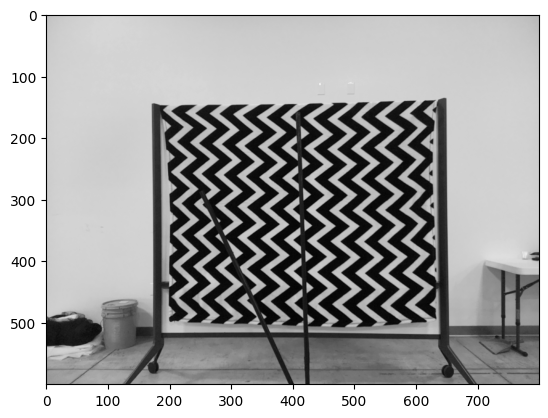
\includegraphics[width=\textwidth]{sections/discussion/zigzag-left-2-obj.png}
            \caption{Left camera image with a single test object.}
            \label{fig:zigzag-2obj-compare:left-double}
        \end{subfigure}
        \hfill
        \begin{subfigure}[b]{0.45\textwidth}
            \centering
            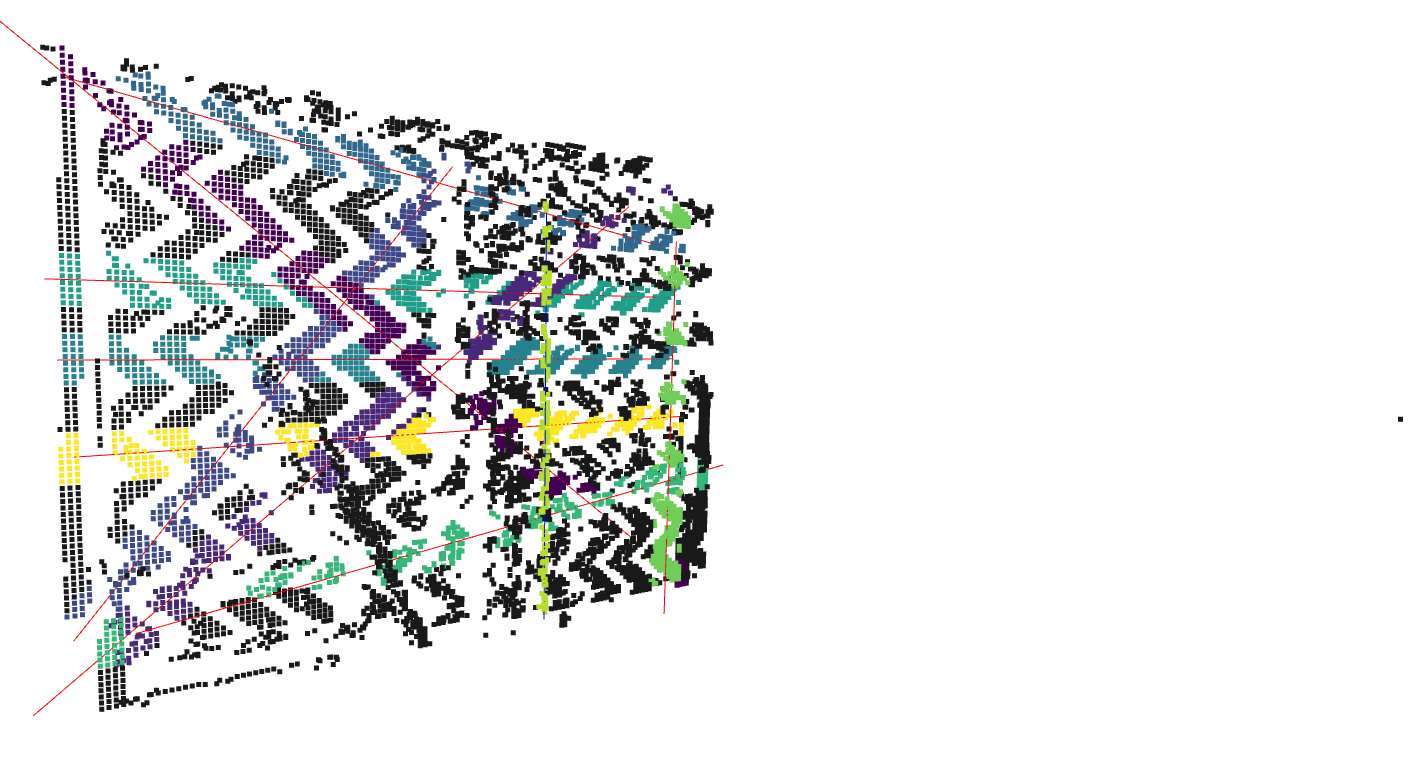
\includegraphics[width=\textwidth]{sections/discussion/zigzag-ptcld-2-obj.png}
            \caption{Point cloud generated from \ref{fig:zigzag-2obj-compare:left-double}, 
                in which the test object has not been detected as a candidate.}
            \label{fig:zigzag-2obj-compare:ptcld-double}
        \end{subfigure}
    \end{subfigure}
    \caption{Sample data from a test with a single object (\ref{fig:zigzag-2obj-compare:left-single} and \ref{fig:zigzag-2obj-compare:ptcld-single})
    in which the object was not correctly detected, and with two objects (\ref{fig:zigzag-2obj-compare:left-double} and \ref{fig:zigzag-2obj-compare:ptcld-double})
    in which the object was correctly detected. Note in \ref{fig:zigzag-2obj-compare:ptcld-double} how the test object is correctly detected, shown as the light green
    points vertically arranged in the center of the point cloud, and the second object is not detected as a candidate line.}
\end{figure}